\subsection{Applications au domaine médical}
Nous venons de voir avec la Table~\ref{tab:etps-sites} que certains entreprises situées dans l'assurance s'intéressaient à XGBoost. Ceci nous a conduit à nous intéresser à l'utilisation qui peut être faite de XGBoost en médecine.

Si encore une fois aucun exemple professionnel n'est ressorti, nous avons pu mettre en avant deux travaux de personnes indépendantes pour réaliser de l'analyse de données médicales avec XGBoost.

\subParagraphe{Amélioration du taux de non-présentation des patients}Ce cas d'application est issu d'un travail personnel qui fut présenté devant des gérants d'agences de santé, et n'a donc pas été réalisé qu'à des fins \og d'études\fg. 

L'idée est ici de détecter des patients qui auraient dû se rendre dans des centres de santé mais ne l'ont pas fait et n'ont ainsi pas été diagnostiqués avant que des symptômes graves ne se déclenchent. 

Dans l'article détaillé \cite{bib:noshow}, l'auteur décrit l'intégralité de son processus de traitement de données. Nous retiendrons pour notre part ici que le modèle utilisé est un simple modèle XGBoost, pour lequel une phase de préparation des données et de recherche des paramètres optimaux a été menée, notament en suivant les bonnes pratiques présentées en Section~\ref{sec:bonnes-pratiques}.

Le modèle obtenu fourni ici des taux de vrais positifs et vrais négatifs compris entre 90 et 92\%, ce qui est considéré comme bon dans le domaine par l'auteur de l'étude. De plus, ce modèle a permis à son auteur de dresser une carte des quartiers à risque concernant ces non-présentations, que nous fournissons en Figure~\ref{fig:noshow}.

\begin{figure}[ht]
	\begin{margincap}
		\centering
		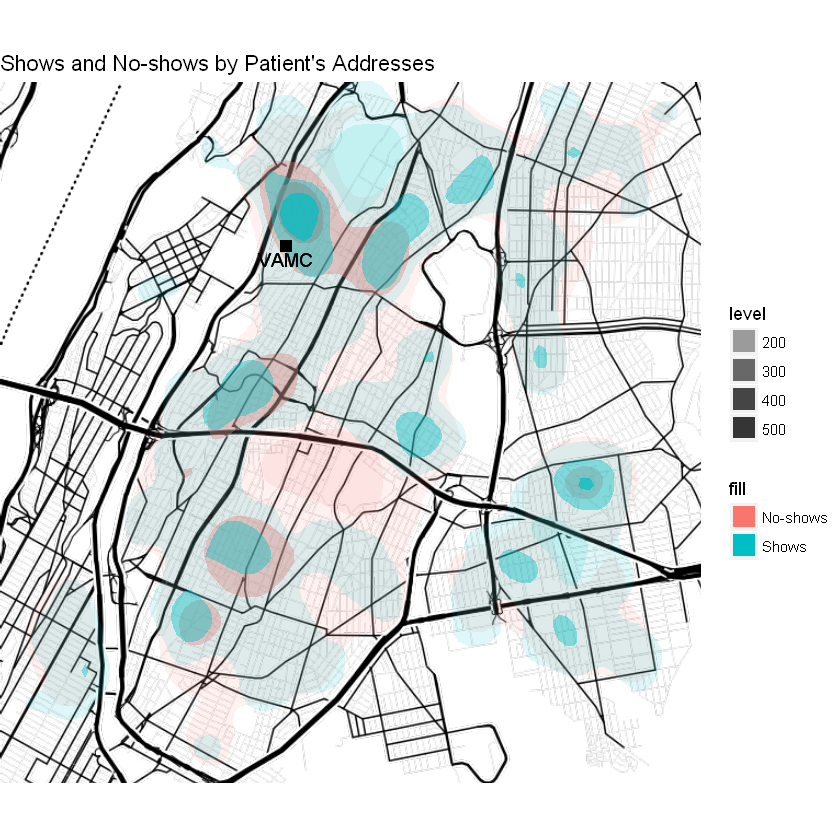
\includegraphics[width=.6\textwidth]{images/Applications/noshow}
		\caption{Carte de risque pour que les patients ne se présente pas au centre de soin établie à partir d'un modèle XGBoost.}
		\label{fig:noshow}
	\end{margincap}
\end{figure}

\subsubsection{Prévision de foyer de grippe}
Ce cas d'application (bien que beaucoup relayé sur Twitter) provient d'un membre de Github réalisant des essais de différentes méthodes de Machine Learning avec R. Dans le cadre de cet essai, l'idée était devoir s'il était possible de créer un modèle pour prévoir les morts dûs à la grippe H7N9 en Chine en 2013.

Après avoir fait des essais avec la plupart des méthodes classiques (Random Forest, Elastic Net et KNN entre autres), l'auteur s'est intéressée aux apports possibles de XGBoost à cette étude.

La conclusion est ici que XGBoot a permis d'obtenir des résultats avec moins d'imprécisions que l'ensemble des autres méthodes, et ce en utilisant les pratiques proposée à la Section~\ref{sec:bonnes-pratiques}\mysidenote{Le code fournit est assez complet, mais le conclusions peu détaillées, en particulier les notations utilisées pour la représentation des résultats. Le lecteur intéressé pourra cependant se rendre à la page en question \cite{bib:flue} pour de plus amples détails.}.

